% Created 2014-07-06 Sun 16:09
\documentclass[presentation,14pt]{beamer}
\usepackage[utf8]{inputenc}
\usepackage[T1]{fontenc}
\usepackage{fixltx2e}
\usepackage{graphicx}
\usepackage{longtable}
\usepackage{float}
\usepackage{wrapfig}
\usepackage{rotating}
\usepackage[normalem]{ulem}
\usepackage{amsmath}
\usepackage{textcomp}
\usepackage{marvosym}
\usepackage{wasysym}
\usepackage{amssymb}
\usepackage{hyperref}
\tolerance=1000
\setbeamertemplate{navigation symbols}{}
\usepackage{courier}
\usepackage{helvet}
\usepackage{listings}
\lstset{
keywordstyle=\color{blue}
, basicstyle=\ttfamily\small
, commentstyle={}
, columns=fullflexible
, showstringspaces=false
, keepspaces=false
, breaklines=true
}
\newcommand{\head}[1]{\begin{center}
\vspace{13mm}\hspace{-1mm}\Huge{{#1}}
\end{center}}
%create template for block without title
\defbeamertemplate{block begin}{notitle}
{
\usebeamerfont{block body}%
\begin{beamercolorbox}[colsep*=.75ex,vmode]{block body}%
\ifbeamercolorempty[bg]{block body}{\vskip-.25ex}{\vskip-.75ex}\vbox{}%
}
\usetheme[height=16mm]{Rochester}
\author{John Wiegley}
\date{4 Jul 2014}
\title{Monads and other abstractions}
\hypersetup{
  pdfkeywords={math monad haskell functional programming},
  pdfsubject={Applying mathematical abstractions to functional programming},
  pdfcreator={Emacs 24.3.1 (Org mode 8.2.6)}}
\begin{document}

\maketitle
\setbeamertemplate{footline}{}
\setbeamercolor{postit}{fg=black,bg=yellow}

\section{Sets}
\label{sec-1}
\begin{frame}[fragile,plain,label=sec-1-1]{HEAD}
\head{Sets}
\end{frame}
\section{Functions}
\label{sec-2}
\begin{frame}[fragile,plain,label=sec-2-1]{HEAD}
\head{Functions}
\end{frame}
\begin{frame}[fragile,label=sec-2-2]{Homomorphisms}
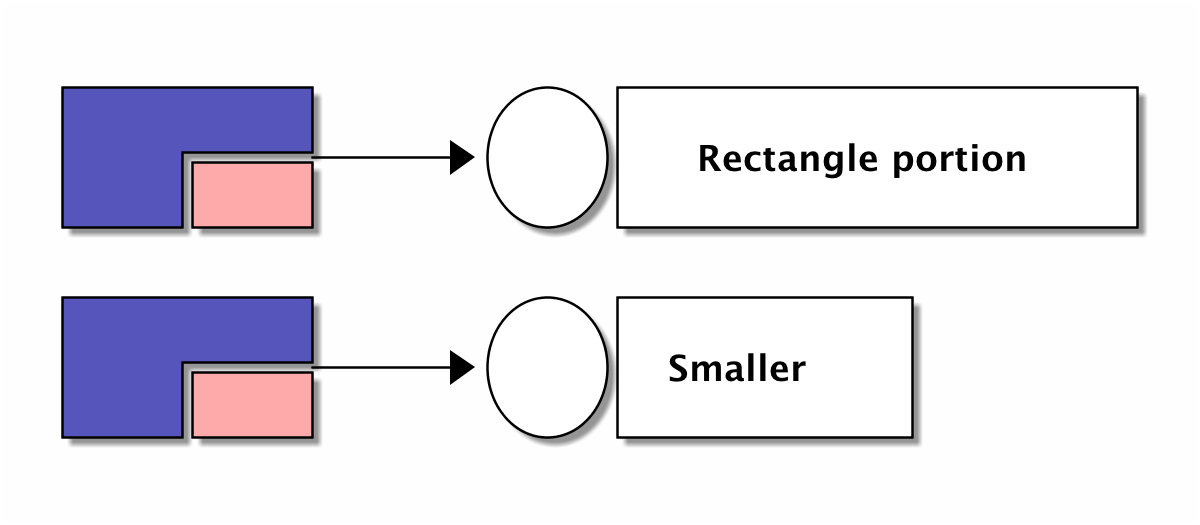
\includegraphics[width=.9\linewidth]{blue.png}
\end{frame}

\begin{frame}[fragile,label=sec-2-3]{Isomorphisms}
\end{frame}
\begin{frame}[fragile,label=sec-2-4]{Endomorphisms}
\end{frame}
\section{Laws}
\label{sec-3}
\begin{frame}[fragile,plain,label=sec-3-1]{HEAD}
\head{Laws}
\end{frame}
\section{Algebras}
\label{sec-4}
\begin{frame}[fragile,plain,label=sec-4-1]{HEAD}
\head{Algebras}
\end{frame}
\section{Algebraic Structures}
\label{sec-5}
\begin{frame}[fragile,plain,label=sec-5-1]{HEAD}
\head{Algebraic Structures}
\end{frame}
\begin{frame}[fragile,label=sec-5-2]{Magmas}
\end{frame}
\begin{frame}[fragile,label=sec-5-3]{Semigroups}
\end{frame}
\begin{frame}[fragile,label=sec-5-4]{Monoids}
\end{frame}
\begin{frame}[fragile,label=sec-5-5]{Groups}
\end{frame}
\section{Type Algebras}
\label{sec-6}
\begin{frame}[fragile,plain,label=sec-6-1]{HEAD}
\head{Type Algebras}
\end{frame}
\section{Equational Reasoning}
\label{sec-7}
\begin{frame}[fragile,plain,label=sec-7-1]{HEAD}
\head{Equational Reasoning}
\end{frame}
\section{Quantification}
\label{sec-8}
\begin{frame}[fragile,plain,label=sec-8-1]{HEAD}
\head{Quantification}
\end{frame}
\section{Parametricity}
\label{sec-9}
\begin{frame}[fragile,plain,label=sec-9-1]{HEAD}
\head{Parametricity}
\end{frame}
\section{Curry-Howard Isomorphism}
\label{sec-10}
\begin{frame}[fragile,plain,label=sec-10-1]{HEAD}
\head{Curry-Howard Isomorphism}
\end{frame}
\section{Free objects}
\label{sec-11}
\begin{frame}[fragile,plain,label=sec-11-1]{HEAD}
\head{Free objects}
\end{frame}
\section{Category Theory}
\label{sec-12}
\begin{frame}[fragile,plain,label=sec-12-1]{HEAD}
\head{Category Theory}
\end{frame}
\section{Functors}
\label{sec-13}
\begin{frame}[fragile,plain,label=sec-13-1]{HEAD}
\head{Functors}
\end{frame}
\section{Applicatives}
\label{sec-14}
\begin{frame}[fragile,plain,label=sec-14-1]{HEAD}
\head{Applicatives}
\end{frame}
\section{Monads}
\label{sec-15}
\begin{frame}[fragile,plain,label=sec-15-1]{HEAD}
\head{Monads}
\end{frame}
\section{Free Monads}
\label{sec-16}
\begin{frame}[fragile,plain,label=sec-16-1]{HEAD}
\head{Free Monads}
\end{frame}
\section{Colophon}
\label{sec-17}
% Emacs 24.3.1 (Org mode 8.2.6)
\end{document}